\documentclass[12pt, a4paper]{report}
%\nonstopmode
\usepackage[english]{babel}
\usepackage[utf8]{inputenc}
\usepackage[T1]{fontenc}
\usepackage[british]{isodate}

\usepackage[usenames]{color}

\usepackage{graphicx}

% TOC
\renewcommand{\thesubsubsection}{\thesubsection.\alph{subsubsection}}


\setcounter{tocdepth}{3}
\setcounter{secnumdepth}{3}

% Margins
\usepackage[hmargin={55pt, 55pt}, vmargin={2.8cm, 2.8cm}]{geometry}

%%% MATH
\usepackage{amsmath}
\usepackage{amssymb}
\usepackage{amsbsy}
\usepackage{amsthm}                % better theorem environments
\usepackage{mathtools}
\usepackage{algorithm}
\usepackage{algpseudocode}
\algnewcommand\algorithmicinput{\textbf{Input:}}
\algnewcommand\Input{\item[\algorithmicinput]}
\algnewcommand\algorithmicoutput{\textbf{Output:}}
\algnewcommand\Output{\item[\algorithmicoutput]}

% Captions
\usepackage[margin=1cm, labelfont=bf]{caption}
\usepackage{subcaption}
\usepackage{hyperref}

\usepackage[inline]{enumitem}

% Citations
\usepackage[numbers]{natbib}

% TikZ
\usepackage{tikz}
\usetikzlibrary{arrows,fit, positioning, shapes,
  calc, fadings, decorations.pathmorphing, hobby}

\tikzset{font=\tiny}
\tikzset{terminal/.style={circle, draw=black, fill=black, text=white}}
\tikzset{steiner/.style={circle, draw=black, fill=white}}
\tikzset{selected/.style={draw=red, ultra thick}}
\tikzset{assignment/.style={draw=red, thin, opacity=0.6}}
\tikzset{root/.style={draw=cyan, ultra thick}}
\tikzset{subgraph/.style={font=\large, text=gray}}
\tikzset{snake it/.style={-stealth,
    decoration={snake, 
      amplitude = .2mm,
    segment length = 2mm,
    post length=0.9mm},decorate}}
\tikzset{snake node/.style={above=1mm,
    midway,
    text width=3cm,
    sloped,
    align=center}}
% Caption types

\DeclareCaptionType{formulation}[Formulation][List of formulations]

% TODO
\usepackage{todonotes}
\presetkeys{todonotes}{size=\tiny}{}

% Theorems
\newtheorem{theorem}{Theorem}[section]
\newtheorem{lemma}{Lemma}[theorem]
\newtheorem{Lemma}{Lemma}[section]
\newtheorem{corollary}{Corollary}[theorem]
\theoremstyle{definition}
\newtheorem{example}{Example}[section]

% Table
\usepackage{multirow}
\usepackage{multicol}
% Ops

\DeclareMathOperator{\id}{id}
\DeclareMathOperator*{\argmin}{argmin}
\DeclareMathOperator*{\argmax}{argmax}
\DeclareMathOperator{\radius}{radius}
\DeclareMathOperator{\pcradius}{pcradius}

% Glossary

\newcommand*{\newdualentry}[5][]{%  
  \newglossaryentry{main-#2}{name={#4},%  
  text={#3\glsadd{#2}},%  
  description={#5},%  
  #1  
  }%  
  \newacronym{#2}{#3\glsadd{main-#2}}{#4}%  
}

\usepackage{glossaries}
\makeglossaries

\newacronym{ilp}{ILP}{integer linear programming}
\newacronym{gsec}{GSEC}{Generalised Subtour Elimination Constraint}
\newacronym{mip}{MIP}{mixed-integer programming}
\newdualentry{pcstp}{PCSTP}
{Prize-Collecting Steiner Tree Problem}
{An NP-Hard graph optimisation problem (\textit{See Section \ref{sec:pcstp}})}
\newacronym{stp}{STP}{Steiner Tree Problem}
\newacronym{sap}{SAP}{Steiner Arborescence Problem}
\newacronym{pcsap}{PCSAP}{Prize-Collecting Steiner Arborescence Problem}
\newacronym{mtp}{MTP}{Median Tree Problem}

\newglossaryentry{delta}
{
  name={\ensuremath{\delta}},
  description={Function: $V \to \mathcal P (V)$, returns the adjacency of
    the input vertex \textit{(See Section \ref{sec:notation:graphs})}},
  sort=pi
}

%%% 
%%% Local Variables:
%%% TeX-master: "report"
%%% reftex-default-bibliography: ("lit.bib")
%%% End:


%\usepackage[titelside, en, nat]{ku-forside}
\usepackage[english, science, titlepage]{ku-frontpage}
%\usepackage{algorithm}
% \usepackage{algcompatible}
% \usepackage{bm}
% \usepackage{bbm}
% \usepackage{algpseudocode}
% \usepackage{arydshln}
% \usepackage[utf8]{inputenc} % æøå
% \usepackage[T1]{fontenc} % mere æøå
% \usepackage{verbatim} % så man kan skrive ren tekst


% \usepackage{graphicx}              % to include figures
% \usepackage{amsfonts}              % for blackboard bold, etc

% \usepackage{bm}
% \usepackage{pgf}
% \usepackage{fancyhdr}
% \usepackage{hyperref}
% \usepackage{stmaryrd}
% \usepackage{mathtools}
% \usepackage{multirow}
% \usepackage{listings}


% various theorems, numbered by section

\newtheorem{thm}{Theorem}[section]
\newtheorem{lem}[thm]{Lemma}
\newtheorem{prop}[thm]{Proposition}
\newtheorem{cor}[thm]{Corollary}
\newtheorem{conj}[thm]{Conjecture}

\newcommand{\nn}{\mathcal{N}}
\newcommand{\uu}{\mathcal{U}}
\newcommand{\bb}{\mathcal{B}}
\newcommand{\ee}{\mathrm{e}}
\newcommand{\rd}[1]{\mathrm{#1}}
\newcommand{\bd}[1]{\mathbf{#1}}  % for bolding symbols
\newcommand{\RR}{\mathbb{R}}      % for Real numbers
\newcommand{\ZZ}{\mathbb{Z}}      % for Integers
\newcommand{\BB}{\mathbb{B}}      % for Booleans
\newcommand{\PP}{\mathbb{P}}      % for Prob
\newcommand{\EE}{\mathbb{E}}      % for Expectation
\newcommand{\II}{\mathbbm{1}}      % for Indicator fun
\newcommand{\NN}{\mathbb{N}}      % for Prob
\newcommand{\col}[1]{\left[\begin{matrix} #1 \end{matrix} \right]}
\newcommand{\comb}[2]{\binom{#1^2 + #2^2}{#1+#2}}

\newcommand{\sint}[1]{\shortintertext{#1}}

\title{Prize-Collecting Steiner Trees}
\author{William Sprent -- \texttt{bsprent@gmail.com}}
\assignment{Master's Thesis} % Findes kun under 'titelside'
\subtitle{From the Perspective of the Prize-Collecting Travelling Salesman Problem}
\date{\today}
\advisor{Supervisors: Pawel Winter}

\begin{document}
\maketitle
~
\begin{abstract}
  The \gls{pcstp} in graphs is an NP-hard optimisation problem which involves
finding a connected subgraph which minimises the total edge cost of
the subgraph summed with all vertex prizes not spanned by the subgraph.
It is a very well researched problem --- not least due to it being one of the
subjects of the \textit{11th DIMACS Implementation Challenge}.

In this master's thesis, we present a comprehensive survey of the research landscape
on the \gls{pcstp}. This involves a thorough look at some of the most interesting
and important algorithms for the \gls{pcstp}. Among the surveyed subjects are
powerful preprocessing routines, the widely cited Goemans-Williamson approximation
algorithm, and two state-of-the-art solvers.

We make use of this survey to consider the relation of the \gls{pcstp} other close
 problems, and take a new look at the younger and much less researched problem, the
\gls{mtp}. This problem is a generalisation of the \gls{pcstp} where instead of paying
static vertex prizes for unspanned vertices, a cost is now paid to \textit{assign}
unspanned vertices to the result subgraph.

For the \gls{mtp} we present a new \acrlong{ilp} formulation as well as a solver which
is able to generate exact solutions to the problem. Furthermore, we present a new
dataset based on previously released datasets for the \gls{pcstp}.

%%% Local Variables:
%%% TeX-master: "report"
%%% reftex-default-bibliography: ("lit.bib")
%%% End:

\end{abstract}

\tableofcontents
\clearpage


\chapter{Introduction}
\section{Background and Motivation}
\label{sec:intro:background}
There exists a family of combinatorial optimisation problems in graphs which involve
finding a subgraph which optimises the trade-off of including a vertex for its prize
(or to avoid paying a penalty) and paying the cost of the edge(s) needed to connect
to it.

These problems generally come with the moniker of \textit{Prize-Collecting}
and were first introduced by \citet*{balas1989prize}
with the introduction of the \textit{\gls{pctsp}}. This problem is a generalisation of
the famous \gls{tsp}, relaxing its Hamiltonian tour constraint by instead applying penalities
to missed vertices and setting a minimum on collected ``prize''.

Perhaps unsurprisingly, this concept of collecting prize spread to another famour optimisation
problem, that is the \gls{stp}. This was done by \citet{Bienstock1993} in conjuction with
defining an approximation algorithm for the \gls{pctsp}. This variant of the \gls{stp},
aptly named the \gls{pcstp}, gained traction --- particularly with the
\textit{11th DIMACS Implementation Challenge}\citep{DIMACS}.

At the onset of writing this thesis, we started off with the goal of surveying research done
on the \gls{pcstp}, and attempting to fill out any holes with methods defined for the older
\gls{pctsp}. This was considered with the assumption that the older problem had
been more covered.
However, it turned out that the \gls{pcstp} had been \textit{far} more covered
by research with multiple exact algorithms
\citep{ljubic2005solving, leitner2016dual, gamrath2017scip},
approximation algorithms \citep{Bienstock1993,goemans1995general,Johnson:2000:PCS:338219.338637},
and primal heuristics \citep{canuto2001local,fu2014knowledge,akhmedov2016divide}
having been already proposed while the \gls{pctsp} had received little such attention
\citep{archetti2014chapter}.

Still wanting to have the \gls{pcstp} as our starting point, we decided to still survery the
problem with the hope that any knowledge gained could be applied somehow. We found an application
for this when running into the \gls{mtp}. The \gls{mtp} is a generalisation of the \gls{pcstp}
which, to the best of our knowledge, has not been explored in the general case. Thus we set out
to apply knowledge from the \gls{pcstp} to the \gls{mtp} to hopefully learn something about
both problems.
\section{Aim and Scope}
The aim of this thesis is two-fold and split in two parts. In the first part, we perform a
survey of the \acrlong{pctsp} where we report, detail, and bring intution to the most interesting
and/or effective methods for solving the \gls{pcstp}.

In the second part, we widen our lenses and look at related problems from the perspective of
the \gls{pcstp}. First superficially, and then with a deep dive in the \acrlong{mtp} for which
we proprose an \gls{ilp} formulation, a new dataset, and a solver.

Overall, we aim to see how well state of the art methods used to solve an NP-hard combinatorial
optimisation problem can be utilised another NP-hard problem when the problems are similar in
formulation.

\section{Related Work}
Besides the work we relay in this thesis, there has been some recent work which is closely related
 to what we present. Particularly, there has been some in surveying the
\acrlong{pcstp} from different angles.

\citet*{rehfeldt2016reduction} present a comprehensive study of all preprocessing routines
for the \gls{pcstp} and the Node-Weighted Steiner Tree Problem. This is similar in scope to
Section~\ref{sec:solving:pre} in this thesis. The reader is encouraged to visit their paper
if they wish to see a more theoretical and comprehensive look at preprocessing routines for
the \gls{pcstp}. We aim to complement this with a slightly more ituitive description of the
routines.

\citet*{sun2018classical} presents a survey of the practical applications of the \gls{pcstp}.
In their thesis, they first perform a short and sweet summary on the historical perspective of
solving the \gls{pcstp}. Their main constribution, however,
is a detailed look at the applications
of the problem in real world scenarios.


\section{Notation}
\label{sec:intro:notation}

Throughout this thesis, we will make repeated use of some shorthand notation, particularly
with respect to graphs and decisions vectors.

\paragraph{Graphs}

We define the adjacency function $\delta : V \to \mathcal{P} (E)$ on undirected graphs as
the function which given the index of a vertex, returns all adjacent edges, that is
$$\delta(i) = \{(i,j) \mid j \in V \wedge (i, j) \in E\}\mathnormal{.}$$
On a directed graph, this is replaced by two functions
$\delta^+ : V \to \mathcal{P} (A)$
and $\delta^-: V \to \mathcal{P} (A)$.
The former returns all vertices, $j$, for which there exists an arc
which starts in the input vertex, $i$, and terminates in $j$, that is
$$\delta^+(i) = \{(i, j) \mid j \in V \wedge (i, j) \in A\}\mathnormal{.}$$
Correspondingly, $\delta^-$ then returns the set,
$$\delta^-(i) = \{(j, i) \mid j \in V \wedge (j, i) \in A\}\mathnormal{.}$$
When we are not interested in adjacent edges, but instead neighbouring vertices,
we may use $\delta(v)$ to mean the set of vertices which are neighbours to $v$.
This will be clear in usage.


When given some subset of vertices, $S \subseteq V$, as input,
$\delta(S)$ returns all edges which span the cut $(S, V \setminus S)$.
Thus we have $\delta : \mathcal{P}(V) \to \mathcal{P}(E)$, with
$$\delta(S) = \{(i,j) \in E \mid i \in S \wedge j \in V \setminus S\}\mathnormal{.}$$
And for directed graphs we have, $\delta^+ : \mathcal{P}(V) \to \mathcal{P}(A)$, with
$$\delta^+(S) = \{(i,j) \in A \mid i \in S \wedge j \in V \setminus S\}\mathnormal{,}$$
and $\delta^- : \mathcal{P}(V) \to \mathcal{P}(A)$, with
$$\delta^-(S) = \{(i,j) \in A \mid i \in V \setminus S \wedge j \in S\}\mathnormal{.}$$

\paragraph{Decision Vectors}

When working with \gls{ilp} models of graph problems, we often need to sum over variables
related to edges or vertices. For example, let $x_{ij}$ be $1$ if the edge $(i,j) \in E$
is part of a solution and $0$ if not, and let $L \subseteq E$ be some subset of edges.
Then the \textit{function} $x : \mathcal{P} (E) \to \NN$ returns the number of edges
 in $L$ which was selected in the solution defined by $x$,
 $$x(L) = \sum_{(i, j) \in L} x_{ij}\mathnormal{.}$$
 If $x_{ij}$ is a real number, then $x(L)$ returns a real number as well.

%%% Local Variables:
%%% TeX-master: "report"
%%% reftex-default-bibliography: ("lit.bib")
%%% End:
\chapter{Background}

\section{Glossary}

\section{Notation}
\label{chap:BG}
\subsection{Graphs}

\paragraph{Adjacency}
\subsection{Decision Variables}

%%% Local Variables:
%%% TeX-master: "report"
%%% reftex-default-bibliography: ("lit.bib")
%%% End:

\chapter{Steiner Trees in Graphs}
\label{chap:steiner-trees}

\section{Steiner Tree Problem}
The Steiner Tree Problem (STP) is defined as follows.
Given an undirected graph
$$G = (V, E, c)$$
 where $c: E \to \RR^+$ defines edge weights, and additionally a set of terminals $N \subseteq V$ then
a Steiner Tree is a tree, $T = (V_T, E_T, c) \subseteq G$, which spans $N$ with minimal cost. We denote vertices which must be part of a feasible solution,
that is $v \in N$, as \textit{terminals}, vertices which are not terminals as \textit{non-terminals},
and vertices which are not required to be part of a solution but are so anyway, that is
$v \in E_T \cap (V \setminus N)$, as \textit{Steiner vertices}.

Furthermore, let $S \subset V$ define a cut in $G$. If we have $S \cap N \neq \emptyset$ and $(V \setminus S) \cap \emptyset$ then we
 call $S$ a \textit{Steiner cut}.

When $N = V$, the STP is equivalent to the Minimum Spanning Tree Problen, and when $|N| = 2$ the STP is equivalent to finding the
shortest path between two vertices. However, while these problems both have polynomial-time solutions, the STP is an NP-Hard problem,
 the decision variant being part of Edmund Karp's original 21 NP-Complete problems \citep{karp1972reducibility}.

\begin{figure}[h]\centering
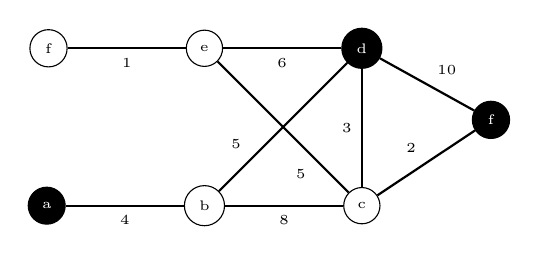
\begin{tikzpicture}[auto, node distance=1.5 cm]
  %Nodes
  \node[terminal] (a) {a};
  \node[steiner] (b) [right=of a] {b};
  \node[steiner] (c) [right=of b] {c};
  \node[terminal] (d) [above =of c] {d};
  \node[steiner] (e) [left=of d] {e};
  \node[steiner] (f) [left=of e] {f};
  \node[terminal] (g) [above right=0.75 and 1.3 of c] {f};
  % Edges
  \begin{scope}[every edge/.style={draw=black, thick}]
    \draw (a) edge node[below]{4} (b);
    \draw (b) edge node[near start]{5} (d);
    \draw (b) edge node[below]{8} (c);
    \draw (c) edge node{3} (d);
    \draw (c) edge node{2} (g);
    \draw (c) edge node[near start]{5} (e);
    \draw (d) edge node{6} (e);
    \draw (d) edge node{10} (g);
    \draw (e) edge node{1} (f);
  \end{scope}
\end{tikzpicture}
\caption{Instance of the Steiner Tree Problem. Terminals are coloured black and non-terminals coloured white.}
\label{fig:stp:01}
\end{figure}

Figure (\ref{fig:stp:01}) shows an instance of the STP with three terminals and four Steiner points. Since vertices
A, C, and D are terminals, they must be spanned by any feasible solution. Figure (\ref{fig:stp:01:feasible}) shows
a feasible solution (which we here denote as a set of edges)
$$E_T = \{(a,b), (b,d), (d,g)\}$$
with cost
$$c(T) = 4 + 5 + 10 = 19\mathnormal{.}$$
However, $T$ is not a Steiner tree as there exists at least one feasible solution with lower cost, i.e. the solution
$$E_{T'} = \{(a,b), (b,d), (d,c), (c,g)\}$$
in Figure (\ref{fig:stp:01:min}) which has cost
$$c(T') = 4 + 5 + 3 + 2 = 14\mathnormal{.}$$
% Suboptimal and Optimal STP solutions 
\begin{figure}[h]\centering
  \begin{subfigure}{0.47\linewidth}
    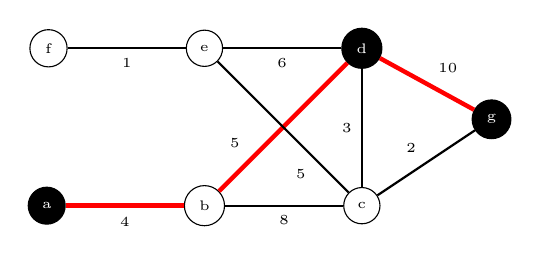
\begin{tikzpicture}[auto, node distance=1.5 cm]
      % Nodes
      \node[terminal] (a) {a};
      \node[steiner] (b) [right=of a] {b};
      \node[steiner] (c) [right=of b] {c};
      \node[terminal] (d) [above =of c] {d};
      \node[steiner] (e) [left=of d] {e};
      \node[steiner] (f) [left=of e] {f};
      \node[terminal] (g) [above right=0.75 and 1.3 of c] {g};
      % Edges
      \begin{scope}[every edge/.style={draw=black, thick}]
        \draw (a) edge[selected] node[below]{4} (b);
        \draw (b) edge[selected] node[near start]{5} (d);
        \draw (b) edge node[below]{8} (c);
        \draw (c) edge node{3} (d);
        \draw (c) edge node{2} (g);
        \draw (c) edge node[near start]{5} (e);
        \draw (d) edge node{6} (e);
        \draw (d) edge[selected] node{10} (g);
        \draw (e) edge node{1} (f);
      \end{scope}
    \end{tikzpicture}
    \caption{Feasible but not optimal.}
    \label{fig:stp:01:feasible}
  \end{subfigure}
  \quad
  \begin{subfigure}{0.47\linewidth}
    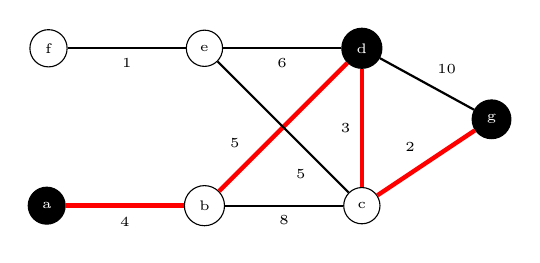
\begin{tikzpicture}[auto, node distance=1.5 cm]
      % Nodes
      \node[terminal] (a) {a};
      \node[steiner] (b) [right=of a] {b};
      \node[steiner] (c) [right=of b] {c};
      \node[terminal] (d) [above =of c] {d};
      \node[steiner] (e) [left=of d] {e};
      \node[steiner] (f) [left=of e] {f};
      \node[terminal] (g) [above right=0.75 and 1.3 of c] {g};
      % Edges
      \begin{scope}[every edge/.style={draw=black, thick}]
        \draw (a) edge[selected] node[below]{4} (b);
        \draw (b) edge node[below]{8} (c);
        \draw (b) edge[selected] node[near start]{5} (d);
        \draw (c) edge[selected] node{3} (d);
        \draw (c) edge[selected] node{2} (g);
        \draw (c) edge node[near start]{5} (e);
        \draw (d) edge node{6} (e);
        \draw (d) edge node{10} (g);
        \draw (e) edge node{1} (f);
      \end{scope}
    \end{tikzpicture}

    \caption{Minimal weight, optimal.}
    \label{fig:stp:01:min}
  \end{subfigure}
  \caption{Solutions to the STP in (\ref{fig:stp:01}). Red edges are part of the solution.}
\end{figure} 

\subsection{ILP Formulations}

\paragraph{Cut Formulation} Let $x$ be a decision vector of length $|E|$ where
$x_{ij} = 1$ implies that $(i,j) \in T$ and $x_{ij} = 0$ implies that $(i,j) \not\in T$,
 and let $c$ be a vector of node-weight s.t. $c_{ij} = c((i,j))$.
Then define the function $x : E \to \ZZ$ as
$$x(E') = \sum_{i,j \in E'} x_{ij}$$
that is, $x(E)$ is equal to the number of selected edges in $E$.
Finally let,
$$\delta(S) = \{(i, j) \mid i \in S \wedge j \in (E \setminus S)\}$$
be all edges which span the cut defined by $S$. Then we can formulate
 the STP as in ILP in terms of cuts (see Formulation (\ref{form:stp:cut})).
 \begin{formulation}[h!]
   \begin{subequations}
     \begin{alignat}{3} %TODO: Find reference for this formulation
       &\underset{x}{\text{minimize}}
       & & c^T x & \\
       & \text{subject to}\quad
       & & x(\delta(S)) \geq 1 \qquad&& \forall S \subset V \label{form:stp:cut:cut}\\
       &&&&& S \cap N \neq \emptyset \nonumber\\
       &&&&& S \cap (V \setminus N) \neq \emptyset \nonumber\\
       &&& x \in \BB. &&
     \end{alignat}\label{form:stp:cut}
   \end{subequations}
   \caption{The \textit{Cut Formulation} of the STP \citep{koch1998solving}.}
 \end{formulation}

 Constraints (\ref{form:stp:cut:cut}) ensures that any feasible solution, $T$,  must span all terminals in $G$, by
 requiring that every Steiner cut in $G$ must be crossed by an edge in $T$. This, combined with objective function
  ensures that any optimal solution to (\ref{form:stp:cut}) must be a Steiner tree in $G$ and vice versa.

\section{Steiner Aborescence Problem}
The Steiner Aborescence Problem (SAP) is the directed version of the Steiner Tree Problem.
Given a \textit{directed} graph,
$$G = (V, A, c)$$
a non-empty terminal set $N \subseteq V$, a root terminal $r \in N$, and arc-weights $c : A \to \RR^+$,
then a Steiner Aborescence, $T \subseteq A$, is an aborescence
in $G$, rooted in $r$, which spans $N$ and has minimal cost.

As with the STP, we denote vertices in $N$ as \textit{terminals}, and any non-terminals spanned by a Steiner Aborescence as
 \textit{Steiner vertices} or \textit{Steiner Points}.
\begin{figure}[h]\centering
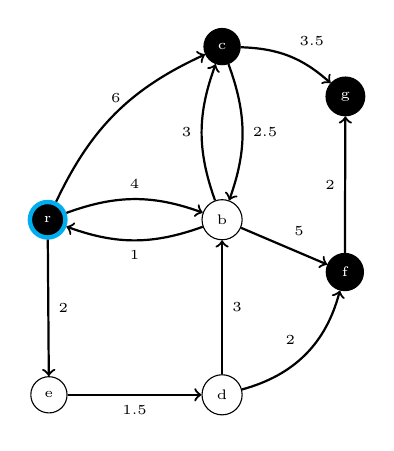
\begin{tikzpicture}[auto, node distance=1.7 cm]
  %Nodes
  \node[terminal, root] (r) at (0,0) {r};
  \node[steiner] (b) [right= of r] {b};
  \node[terminal] (c) [above= of b] {c};
  \node[steiner] (d) [below= of b] {d};
  \node[steiner] (e) [left= of d] {e};
  \node[terminal] (f) [above right= of d] {f};
  \node[terminal] (g) [above right= of b] {g};
  % Edges
  \begin{scope}[every edge/.style={draw=black, thick}]
    \draw[->] (r) edge [bend left=20] node[above]{4} (b);
    \draw[<-] (r) edge [bend right=20] node[below]{1} (b);
    \draw[->] (r) edge [bend left=20] node[above]{6} (c);
    \draw[->] (r) edge  node{2} (e);
    \draw[->] (b) edge [bend left=20] node{3} (c);
    \draw[<-] (b) edge [bend right=20] node[swap]{2.5} (c);
    \draw[<-] (b) edge  node{3} (d);
    \draw[->] (b) edge  node{5} (f);
    \draw[->] (c) edge [bend left=20] node{3.5} (g);
    \draw[<-] (d) edge  node{1.5} (e);
    \draw[->] (d) edge [bend right] node{2} (f);
    \draw[->] (f) edge node{2} (g);
  \end{scope}
\end{tikzpicture}
\caption{Instance of the Steiner Aborescence Problem. Terminals are coloured black, non-terminals are coloured white, and the root terminal
  has a blue outline.}
\label{fig:sap:01}
\end{figure}

Figure (\ref{fig:sap:01}) shows an instance of the SAP with four terminals. Figure (\ref{fig:sap:01:opt}) shows a Steiner Aborescence in (\ref{fig:sap:01})
with cost $c(T) = 13.5$. It is worth noting that since all arcs must point away from the root in an aborescence, while the path $c, b, r$  has
 lower cost than the arc $(r, c)$, it cannot be part of a solution. Similarly, solutions to the SAP in the same graph but with root $c$ have lower cost.

\begin{figure}[h]\centering
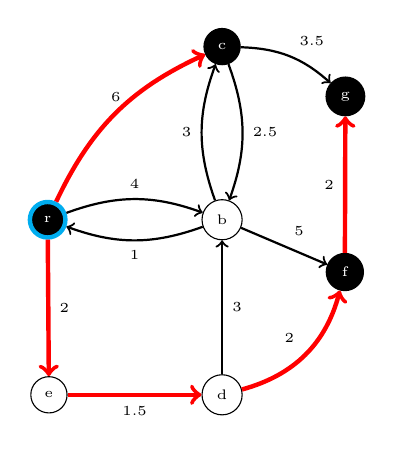
\begin{tikzpicture}[auto, node distance=1.7 cm]
  %Nodes
  \node[terminal, root] (r) at (0,0) {r};
  \node[steiner] (b) [right= of r] {b};
  \node[terminal] (c) [above= of b] {c};
  \node[steiner] (d) [below= of b] {d};
  \node[steiner] (e) [left= of d] {e};
  \node[terminal] (f) [above right= of d] {f};
  \node[terminal] (g) [above right= of b] {g};
  % Edges
  \begin{scope}[every edge/.style={draw=black, thick}]
    \draw[->] (r) edge [bend left=20] node[above]{4} (b);
    \draw[<-] (r) edge [bend right=20] node[below]{1} (b);
    \draw[->] (r) edge [bend left=20, selected] node[above]{6} (c);
    \draw[->] (r) edge [selected] node{2} (e);
    \draw[->] (b) edge [bend left=20] node{3} (c);
    \draw[<-] (b) edge [bend right=20] node[swap]{2.5} (c);
    \draw[<-] (b) edge  node{3} (d);
    \draw[->] (b) edge  node{5} (f);
    \draw[->] (c) edge [bend left=20] node{3.5} (g);
    \draw[<-] (d) edge [selected, selected] node{1.5} (e);
    \draw[->] (d) edge [bend right, selected] node{2} (f);
    \draw[->] (f) edge [selected] node{2} (g);
  \end{scope}
\end{tikzpicture}
\caption{Steiner Aborescence in (\ref{fig:sap:01}) with cost $13.5$.}
\label{fig:sap:01:opt}
\end{figure}

The SAP is relevant mainly due to a tendency of reformulating the undirected STP into the SAP \citep{koch1998solving}, as well as reformulating
the PCSTP into the SAP \citep{gamrath2017scip, Ljubic:2004:memetic} and
prize-collecting variants of the SAP \citep{leitner2016dual, ljubic2005solving} before stating them as integer programs. This is due to results which show that LP relaxations of
 directed Steiner Tree Problem variants behave better than undirected variants \citep{Chopra:1994}.

\subsection{Reduction from Other Variants}

\subsubsection{Steiner Tree Problem}
\begin{figure}[h]\centering
  \begin{subfigure}{0.47\linewidth}
    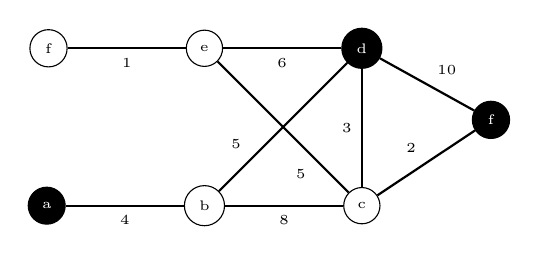
\begin{tikzpicture}[auto, node distance=1.5 cm]
      % Nodes
      \node[terminal] (a) {a};
      \node[steiner] (b) [right=of a] {b};
      \node[steiner] (c) [right=of b] {c};
      \node[terminal] (d) [above =of c] {d};
      \node[steiner] (e) [left=of d] {e};
      \node[steiner] (f) [left=of e] {f};
      \node[terminal] (g) [above right=0.75 and 1.3 of c] {f};
      % Edges
      \begin{scope}[every edge/.style={draw=black, thick}]
        \draw (a) edge node[below]{4} (b);
        \draw (b) edge node[near start]{5} (d);
        \draw (b) edge node[below]{8} (c);
        \draw (c) edge node{3} (d);
        \draw (c) edge node{2} (g);
        \draw (c) edge node[near start]{5} (e);
        \draw (d) edge node{6} (e);
        \draw (d) edge node{10} (g);
        \draw (e) edge node{1} (f);
      \end{scope}
    \end{tikzpicture}
    \caption{Problem Instance (\ref{fig:stp:01})}
  \end{subfigure}
  \begin{subfigure}{0.47\linewidth}
    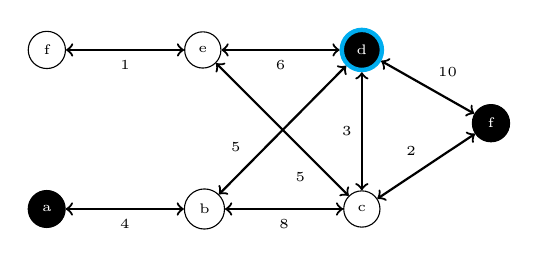
\begin{tikzpicture}[auto, node distance=1.5 cm]
      % Nodes
      \node[terminal] (a) {a};
      \node[steiner] (b) [right=of a] {b};
      \node[steiner] (c) [right=of b] {c};
      \node[terminal, root] (d) [above =of c] {d};
      \node[steiner] (e) [left=of d] {e};
      \node[steiner] (f) [left=of e] {f};
      \node[terminal] (g) [above right=0.75 and 1.3 of c] {f};
      % Edges
      \begin{scope}[every edge/.style={draw=black, thick}]
        \draw[<->] (a) edge node[below]{4} (b);
        \draw[<->] (b) edge node[near start]{5} (d);
        \draw[<->] (b) edge node[below]{8} (c);
        \draw[<->] (c) edge node{3} (d);
        \draw[<->] (c) edge node{2} (g);
        \draw[<->] (c) edge node[near start]{5} (e);
        \draw[<->] (d) edge node{6} (e);
        \draw[<->] (d) edge node{10} (g);
        \draw[<->] (e) edge node{1} (f);
      \end{scope}
    \end{tikzpicture}
    \caption{Instance (\ref{fig:stp:01}) as a SAP instance. Root node is coloured blue.}
  \end{subfigure}
  \caption{Reduction from STP to SAP.}
  \label{fig:stptosap}
\end{figure}

\subsubsection{Prize-Collecting Steiner Tree Problem}

\subsection{ILP Formulations}
\section{Prize-Collecting Steiner Tree Problem}
Given an undirected graph
$$G = (V, E, c, p)$$
where $c: E \to \RR^+$ defines edge weights,
and $p: V \to \RR^+$ defines vertex \textit{prizes}, then the solution to the \textit{Prize-Collecting
  Steiner Tree Problem} (PCSTP) is a tree
$$T = (V_T, E_T, c, p) \subseteq G$$
which minimizes
$$GW(T) = \sum_{(i,j) \in E_T} c_{ij} + \sum_{v\in (V_T \setminus V)} p_v$$
which is also known as the {\textit{Goemans-Williamson Minimization Problem}}.

The PCSTP can equilvalently be stated as the {\textit{Net Worth Maximization Problem}} \citep{Johnson:2000:PCS:338219.338637},
$$NW(T) = \sum_{v \in V_T} p_v - \sum_{(i,j) \in E_T} c_{ij} \mathnormal{.}$$
In the context of the PCSTP, We denote vertices with nonzero prize as \textit{terminals}, giving the terminal set
$$N = \{v \mid p_v > 0\} \subseteq V\mathnormal{.}$$

\begin{figure}[h]\centering
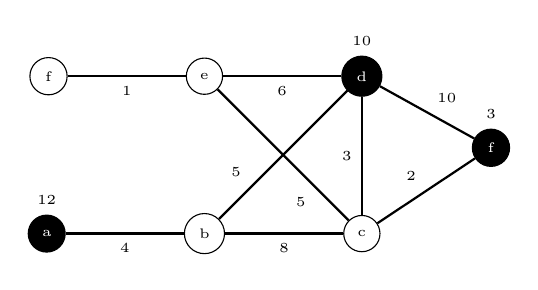
\begin{tikzpicture}[auto, node distance=1.5 cm]
  %Nodes
  \node[terminal, label={12}] (a) {a};
  \node[steiner] (b) [right=of a] {b};
  \node[steiner] (c) [right=of b] {c};
  \node[terminal, label={10}] (d) [above =of c] {d};
  \node[steiner] (e) [left=of d] {e};
  \node[steiner] (f) [left=of e] {f};
  \node[terminal, label={3}] (g) [above right=0.75 and 1.3 of c] {f};
  % Edges
  \begin{scope}[every edge/.style={draw=black, thick}]
    \draw (a) edge node[below]{4} (b);
    \draw (b) edge node[near start]{5} (d);
    \draw (b) edge node[below]{8} (c);
    \draw (c) edge node{3} (d);
    \draw (c) edge node{2} (g);
    \draw (c) edge node[near start]{5} (e);
    \draw (d) edge node{6} (e);
    \draw (d) edge node{10} (g);
    \draw (e) edge node{1} (f);
  \end{scope}
\end{tikzpicture}
\caption{Instance of the Prize-Collecting Steiner Tree Problem. Terminals are coloured black and non-terminals coloured white.}
\label{fig:pcstp:01}
\end{figure}

Figure (\ref{fig:pcstp:01}) shows an instance, $G$, of the PCSTP created by assigning prizes to the terminals of the STP instance, $G_{STP}$, in Figure (\ref{fig:stp:01}).
Figure (\ref{fig:pcstp:01})
shows an optimal solution, $T = (V_T, E_T)$, to $G$. An interesting observation is that
$T$ is a sub-graph of the solution in Figure (\ref{fig:stp:01:min}) to $G_{STP}$.
In fact, if we were to modify $G_{STP}$ by setting its terminal set to the vertices spanned
by $T$, that is we define $G'_{STP} =  G_{STP}$ where  $N_{G'_{STP}} = V_T$, then $T$ is a Steiner
tree in $G'_{STP}$. In other words, we can describe the search space of the PCSTP
 as the set of all Steiner trees in a graph $G$.

\begin{figure}[h]\centering
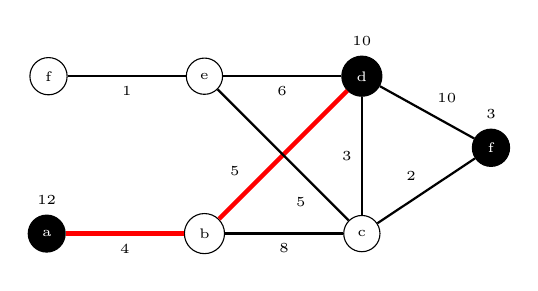
\begin{tikzpicture}[auto, node distance=1.5 cm]
  %Nodes
  \node[terminal, label={12}] (a) {a};
  \node[steiner] (b) [right=of a] {b};
  \node[steiner] (c) [right=of b] {c};
  \node[terminal, label={10}] (d) [above =of c] {d};
  \node[steiner] (e) [left=of d] {e};
  \node[steiner] (f) [left=of e] {f};
  \node[terminal, label={3}] (g) [above right=0.75 and 1.3 of c] {f};
  % Edges
  \begin{scope}[every edge/.style={draw=black, thick}]
    \draw (a) edge[selected] node[below]{4} (b);
    \draw (b) edge[selected] node[near start]{5} (d);
    \draw (b) edge node[below]{8} (c);
    \draw (c) edge node{3} (d);
    \draw (c) edge node{2} (g);
    \draw (c) edge node[near start]{5} (e);
    \draw (d) edge node{6} (e);
    \draw (d) edge node{10} (g);
    \draw (e) edge node{1} (f);
  \end{scope}
\end{tikzpicture}
\caption{Optimal solution to (\ref{fig:pcstp:01})\textnormal{.}}
\label{fig:pcstp:01:opt}
\end{figure}

Unsurprisingly, the PCSTP is an NP-Hard problem. It is a generalisation of the STP. Any instance of
the STP with graph $G = (V, E, c)$ and terminal set $N$ can be reduced to an instance of the PCSTP
with graph $G' = (V, E, c, p)$ where
where
$$p_v =
\begin{cases}
  \infty & v \in N\mathnormal{,} \\
  0 & \mathnormal{otherwise.}
\end{cases}$$
Any optimal solution to $G'$ is then a Steiner tree in $G$ and vice versa.
\subsection{ILP Formulations}
%%% Local Variables:
%%% TeX-master: "report"
%%% reftex-default-bibliography: ("lit.bib")
%%% End:

\chapter{Solving the Prize-Collecting Steiner Tree Problem}
\label{chap:solving}
\section{Preprocessing}
Applying preprocessing routines to heavily reduce input graphs is a common technique which has been proven succesful in many cases both for instances of the STP
\citep{koch1998solving}
and instances of the PCSTP
\citep{ljubic2005solving, gamrath2017scip}. %TODO: MORE
These routines make use of proven invariants to remove and contract edges as well as choose edges before applying the any main procedure.
A set of common preprocessing routines are applied in different manners in literature, mainly differentiated by:
\begin{enumerate}[label=\alph*)]
\item which routines to apply,
\item in which order, and
\item when to recursively apply routines and how many times.
\end{enumerate}
Preprocessing routines can be very effective. For example, the preprocesing routine presented by \cite{koch1998solving} for the STP removes
up to 98\% of edges in some instances. In this section, we will first give a full overview of existing preprocessing methods for the PCSTP,
 including proofs of validity,
 and then summarize their usage in recent literature.

 In the following, we will denote any edge or vertex (or part of a graph) as \textit{redundant} if there exists an optimal solution
  which does not contain it, and we say that a 
  transformation to a problem instance is \textit{valid} when produces an equivalent problem, that is a problem which has the same optimal
  value and in which solutions map back to the original problem.

 \subsection{Local Reduction Tests}
 The first type of reductions we will look at, we will named \textit{local} reduction tests. These are tests which only require knowledge
 of the neighbourhood of a couple of vertexes in the graph, and perhaps simple global information such as maximum prize. As such, the tests
 presented in this section are generally of low computational cost, allowing for testing a full graph in linear time.

 Note that the first tests presented (NTD1, NTD2, TD1, TD2) are known collectively
 in recent literature as \textit{Degree Tests}, for example in \cite{rehfeldt2016reduction}.
\subsubsection{Non-Terminals of Degree 1}
\label{sec:red:test:deg1}
Let $G = (V, E, c, p)$ be a PCST instance and let $v \in V$ be any non-terminal with degree 1, then
 clearly -- since edges have positive weights -- $v$ can not be part of an optimal solution. Thus $v$ is redundant. In other words,
 all vertices in the set
 $$\{v \mid v \in V \setminus N \wedge |\delta(v)| = 1\}$$
 are redundant and it is valid to remove them from $G$ along with their adjacent edges.

\begin{figure}[h]\centering
    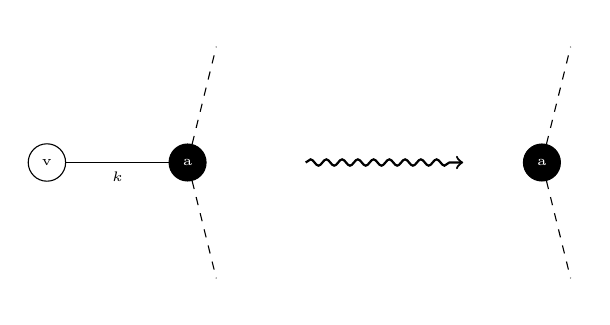
\begin{tikzpicture}[auto, node distance=1.3 cm]
      % Pre
      \begin{scope}[shift={(-0.5,0)}]
        \node[terminal] (a) at (0, 0) {a};
        \node[steiner] (b) [left=of a] {v};
        \node (sg) [above right = 1.3 and 0.1 of a] {};
        \node (sg2) [below right= 1.3 and 0.1 of a] {};

        %Edges
        \draw (a) edge node {$k$} (b);
        \draw[dashed] (a) to (sg);
        \draw[dashed] (a) to (sg2);
      \end{scope}

      \draw [->,decorate, thick,
      decoration={snake,amplitude=.4mm,segment length=2mm,post length=1mm}]
      (1.0,0) -- (3,0);
      % Post      
      \begin{scope}[shift={(4cm, 0)}]

        \node[terminal] (a) at (0, 0) {a};
        \node (sg) [above right = 1.3 and 0.1 of a] {};
        \node (sg2) [below right= 1.3 and 0.1 of a] {};

        %Edges
        \draw[dashed] (a) to (sg);
        \draw[dashed] (a) to (sg2);
      \end{scope}

  \end{tikzpicture}
  \caption{Removing a non-terminal with degree 1.}
  \label{fig:red:test:deg1}
\end{figure}

 While this reduction test is originally stated for the STP \citep{hwang1992steiner}, it is also applicable to the PCSTP. Figure (\ref{fig:red:test:deg1})
  shows an example of removing a degree 1 non-terminal.

  \subsubsection{Non-Terminals of Degree 2}
    \label{fig:red:test2}
\todo{These two sections probably use too different methods in defining their reductions}
    Similarly, let $G = (V,E,c,p)$ be an instance of the PCSTP, let $v \in G$ be a non-terminal with degree $|\delta(v)| = 2$, and let
    $u$ and $w$ be the two vertices adjacent to $v$. Then we can obtain a reduced, equivalent graph,
    $$G' = (V', E', c', p)$$
    where
    $$V' = V - v \mathnormal{,}$$
    $$E' = (E \setminus \{(u,v),(w,v)\}) \cup \{(u,w)\}\mathnormal{,}$$
    and
    $$c_{uw} =
    \begin{cases}
      \min(c_{uw}, c_{uv} + c_{vw}) & (u,w) \in E\mathnormal{,} \\
      c_{uv} + c_{vw} & \text{otherwise.}
    \end{cases}$$

    In other words, if $c_{uv} + c_{vw} <  c_{uw}$ then $(u,w)$ is redundant, can be removed, and $v$ and its edges
    can be contracted to a single edge.
    Otherwise $v$ and its edges are redundant and can be removed. Figure (\ref{fig:red:test:deg2})
    shows an example this reduction test.

\begin{figure}[h!]\centering
    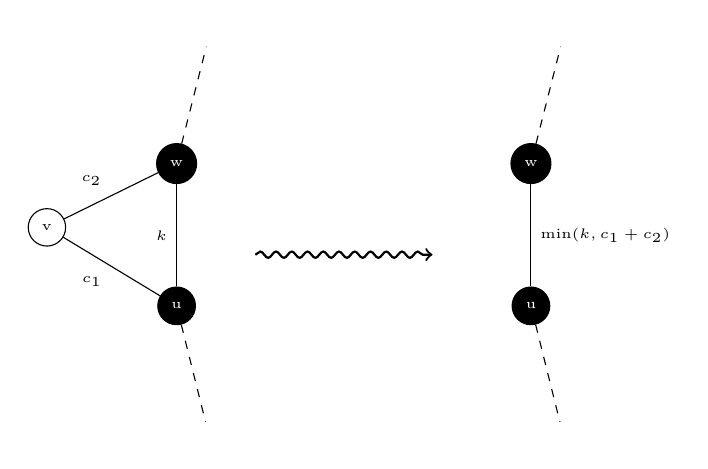
\begin{tikzpicture}[auto, node distance=1.3 cm]
      % Pre
      \begin{scope}
        \node[terminal] (a) at (0, -0.65) {u};
        \node[terminal] (b) [above=of a] {w};
        \node[steiner] (c) [above left= 0.65 and 1.3 of a] {v};
        \node (sg) [above right = 1.3 and 0.1 of b] {};
        \node (sg2) [below right= 1.3 and 0.1 of a] {};

        %Edges
        \draw (a) edge node {$k$} (b);
        \draw (a) edge node {$c_1$} (c);
        \draw (b) edge node[swap] {$c_2$} (c);
        \draw[dashed] (b) to (sg);
        \draw[dashed] (a) to (sg2);
      \end{scope}

      \draw [->,decorate, thick,
      decoration={snake,amplitude=.4mm,segment length=2mm,post length=1mm}]
      (1,0) -- (3.25,0);
      % Post      
      \begin{scope}[shift={(4.5cm, 0)}]
        \node[terminal] (a) at (0, -0.65) {u};
        \node[terminal] (b) [above=of a] {w};
        \node (sg) [above right = 1.3 and 0.1 of b] {};
        \node (sg2) [below right= 1.3 and 0.1 of a] {};

        %Edges
        \draw (a) edge node[swap] {$\min(k, c_1 + c_2)$} (b);
        \draw[dashed] (b) to (sg);
        \draw[dashed] (a) to (sg2);
      \end{scope}

  \end{tikzpicture}
  \caption{Removing a non-terminal with degree 2.}
  \label{fig:red:test:deg2}
\end{figure}

This test is another example of a reduction test for the STP which can by directly applied to
 the PCSTP.
\subsubsection{Terminals of Degree 1}
\label{sec:red:test:tdeg1}
\todo[inline]{Write this section. It's very clear.}
\begin{figure}[h!]\centering
    \begin{tikzpicture}[auto, node distance=1.3 cm]
      % Pre
      \begin{scope}[shift={(-0.5,0)}]
        \node[terminal, label={$p_a$}] (a) at (0, 0) {a};
        \node[terminal, label={$p_v$}] (b) [left=of a] {v};
        \node (sg) [above right = 1.3 and 0.1 of a] {};
        \node (sg2) [below right= 1.3 and 0.1 of a] {};

        %Edges
        \draw (a) edge node {$k$} (b);
        \draw[dashed] (a) to (sg);
        \draw[dashed] (a) to (sg2);
      \end{scope}

      \draw [->,decorate, thick,
      decoration={snake,amplitude=.4mm,segment length=2mm,post length=1mm}]
      (1.0,1) -- node [above=1mm,midway,text width=3cm, sloped, align=center] {$k\geq p_v$}
      (3,2);
      % Post      
      \begin{scope}[shift={(6cm, 3cm)}]

        \node[terminal, label=right:{$p_a$}] (a) at (0, 0) {a};
        \node[terminal, label={$p_v$}] (b) [left=of a] {v};
        
        \node (sg) [above right = 1.3 and 0.1 of a] {};
        \node (sg2) [below right= 1.3 and 0.1 of a] {};

        %Edges
        \draw[dashed] (a) to (sg);
        \draw[dashed] (a) to (sg2);
      \end{scope}

      \draw [->,decorate, thick,
      decoration={snake,amplitude=.4mm,segment length=2mm,post length=1mm}]
      (1.0,-1) -- node [above=1mm,midway,text width=3cm, sloped, align=center] {$k < p_v$}
      (3,-2);

      % Post2      
      \begin{scope}[shift={(6cm, -3cm)}]
        \node[terminal, label=right:{$p_a + (p_v - k)$}] (a) at (0, 0) {a};
        \node[terminal, label={$p_v$}] (b) [left=of a] {v};

        \node (sg) [above right = 1.3 and 0.1 of a] {};
        \node (sg2) [below right= 1.3 and 0.1 of a] {};

        %Edges
        \draw[dashed] (a) to (sg);
        \draw[dashed] (a) to (sg2);
      \end{scope}

  \end{tikzpicture}
  \caption{Removing the edge connected a terminal of degree 1.}
  \label{fig:red:test:deg1}
\end{figure}

\subsubsection{Terminals of Degree 2}


\subsubsection{Minimum Adjacency}
Again defined in \cite{duin1989reduction} for the STP, the \textit{minimum adjacency test}
(also known as the \textit{$V \setminus K$ test}) is a reduction test which contracts adjacent
terminals as shown in Figure (\ref{fig:red:test:ma}).
 
\begin{figure}[h!]\centering
    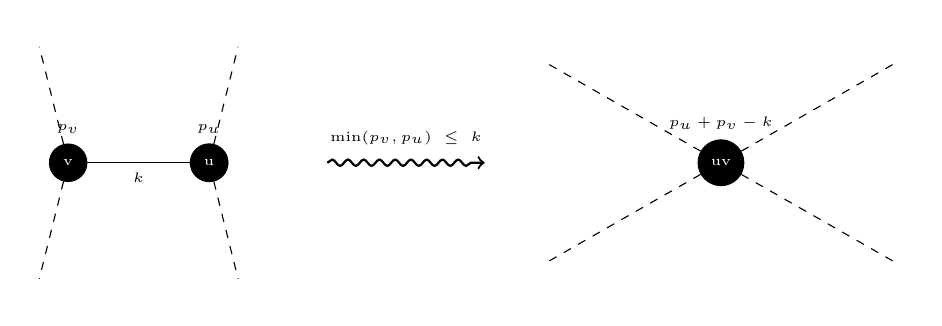
\begin{tikzpicture}[auto, node distance=1.3 cm]
      % Pre
      \begin{scope}[shift={(-0.5,0)}]
        \node[terminal, label={$p_u$}] (u) at (0, 0) {u};
        \node[terminal, label={$p_v$}] (v) [left=of u] {v};
        \node (sgu) [above right = 1.3 and 0.1 of u] {};
        \node (sgu2) [below right= 1.3 and 0.1 of u] {};

        \node (sgv) [above left = 1.3 and 0.1 of v] {};
        \node (sgv2) [below left= 1.3 and 0.1 of v] {};

        %Edges
        \draw (u) edge node {$k$} (v);
        \draw[dashed] (u) to (sgu);
        \draw[dashed] (u) to (sgu2);
        \draw[dashed] (v) to (sgv);
        \draw[dashed] (v) to (sgv2);
      \end{scope}

      \draw [->,decorate, thick,
      decoration={snake,amplitude=.4mm,segment length=2mm,post length=1mm}]
      (1.0,0) -- node [above=1mm,midway,text width=3cm, sloped, align=center] {$\min(p_v, p_u) \leq k$}
      (3,0);
      % Post      
      \begin{scope}[shift={(6cm, 0cm)}]
        \node[terminal, label={$p_u + p_v - k$}] (u) at (0, 0) {uv};
        \node (sgu) [above right = 1. and 2.0 of u] {};
        \node (sgu2) [below right= 1. and 2.0 of u] {};
        \node (sgv) [above left = 1. and 2.0 of u] {};
        \node (sgv2) [below left= 1. and 2.0 of u] {};

        %Edges
        \draw[dashed] (u) to (sgu);
        \draw[dashed] (u) to (sgu2);
        \draw[dashed] (u) to (sgv);
        \draw[dashed] (u) to (sgv2);
      \end{scope}

  \end{tikzpicture}
  \caption{Minimum adjacency test.}
  \label{fig:red:test:ma}
\end{figure}

\begin{theorem}[Minimum Adjacency]
  Let $u$ and $v$ be adjacent terminals in $G$. If we have
  $$\min(p_u, p_v) \geq c_{uv}$$
  and
  $$c_{uv} = \min_{(u, w) \in E}c_{uw}$$
  then it is valid to contract $u$ and $v$.
\end{theorem}
\begin{proof}
  It can be shown that any solution $T$ for the PCSTP problem defined by a graph $G$
  which contains $u$ but not $(u,v)$ can
  be transformed into a solution $T'$ which contains $(u,v)$ where $c(T') \leq c(T)$.

  \paragraph{Case 1: $v \in V_T$}
  Let $(u, w) \in E_T$ be the first edge in the simple path from $u$ to $v$. By assumption, we
  have that $c_{uv} \leq c_{uw}$, and the tree $T'$ constructed by removing $(u,w)$ from $T$ and
  adding $(u,v)$ has cost
  $$c(T') = c(T) - c_{uw} + c_{uv} \leq T\mathnormal{.}$$
  \paragraph{Case 2: $v  \not\in V_T$}
  Let $T'$ be the tree obtained by adding $(u,v)$ to $T$. As per the assumption that $\min(p_u, p_v) \geq c_{uv}$,
  we have that $T'$ has cost,
  $$c(T') = c(T) + c_{uv} - p_{uv} \leq c(T)\mathnormal{.}$$
\end{proof}

\subsubsection{Unconnected Dominated Vertex}


\subsection{Steiner Distance Reduction Tests}
% $$d(u,v) = \min \{ c(P) \mid P \in \mathcal{P}_{uv}\}$$
More complex tests can be described in terms
of the concepts Steiner distance and Bottleneck distance. These were originally stated for
the STP in, amongst others, \cite{duin1989edge,duin1989reduction} and later
adapted for the PCSTP in \cite{uchoa2006reduction}.

First we must make some definitions.
If $P = (..., u, ..., w, ...)$ is a simple path in $G$, then $P_{uw}$ is
the subpath in $P$ starting at vertex $u$ and ending in vertex $w$,
\todo{Some of this should probably go in a notations section}
that is $P_{u,w} = (u, ...,w)$. Then we define the \textit{Steiner distance} of
 $P_{uw}$ as,

 $$sd(P_{uw}) = \sum_{(i,j) \in E(P_{u,w})} c_{i,j} -
 \sum_{v \in V(P) \setminus \{u,w\}} p_{v}\mathnormal{.}$$
 We then denote the Steiner distance of a simple path, $P$, as the maximal Steiner
 distance found among subpaths of $P$,
 $$sd(P) = \max_{u,w \in P} sd(P_{uw})\mathnormal{.}$$
 Let $\mathcal{P}_{uw}$ be the set of all simple paths
 connecting vertices $u$ and $w$ in
 $G$, then we denote the \textit{bottleneck distance} between $u$ and $w$ as minimal Steiner
  distance among paths in $\mathcal{P}_{uw}$,
  $$B(u,w) = \min_{P \in  \mathcal{P}_{uw}} sd(P)\mathnormal{.}$$
  The bottleneck distance is a measure of the worst case \textit{additional cost}
  \todo{Make decision on whether I should replicated proofs for claims like this.}
 of connecting
 two disjoint subgraphs containing vertices $u$ and $v$ respectively in $G$.

  \missingfigure{Some visual intuition on the bottleneck distance}

  Finally, we denote the bottleneck distance between vertices $u$ and $w$ \textit{excluding}
  the edge $e$ as,
  $$B(u,w)^{-e} = \min_{P \in  \mathcal{P}_{uw}, e \not \in P} sd(P)\mathnormal{.}$$


 \cite{uchoa2006reduction} shows that calculating the bottleneck distance
 is an NP hard problem by reduction from the Hamiltonian Path problem. Hence,
 exactly calculating the bottleneck distance is infeasible. However, \cite{uchoa2006reduction}
 also claims that existing heuristics are fast and give strong upper bounds.
 \subsubsection{Special Distance}
 \label{sec:red:test:sd}
 Using the PCSTP version of the Steiner and bottleneck distances, \cite{uchoa2006reduction} proves
  the validity of the more general \textit{special distance test}.
 \begin{theorem}[Special Distance Test]
 Consider any edge $(u,v) \in E$. If we have
 $$B(u,v)^{-(u,v)} \leq c_{uv}$$
 then $(u,v)$ is redundant.
\end{theorem}
 \begin{proof}
   Let $T  \subseteq G$ be an optimal solution to the PCSTP in graph $G$
   where we have
   $$B(u,v)^{-(u,v)} \leq c_{uv}$$
   for some edge $(u,v) \in E_T$, and let $(T_1, T_2)$ be the cut bridged
   by $(u,v)$.

   Consider then the simple path $P \in \mathcal{P}_{uv}$ from $u$ to $v$ which doesn't
    contain $(u,v)$ and has
   $$sd(P) = B(u,v)^{-(u,v)}\mathnormal{.}$$

   Since $T$ is a tree, and $P$ by definition doesn't contain the edge $(u,v)$
   then we must have that $P$ consists of a subpath contained in $T_1$, followed by
   a subpath not contained in $T$, followed by a subpath contained in $T_2$.
   In other words, we have,
   $$P = (u, P_1, w, P_2, z, P_3, v)$$
   as shown in Figure \ref{fig:red:test:sd:thm}.

   Then by definition we have,
   $$sd(P_2) \leq sd(P) = B(u,v)^{-(u,v)} \leq c_{uv}$$
   and we construct another solution $T'$ by replacing $(u,v)$ with the
   vertices and edges in $P_2$ which has cost
   $$c(T') = c(T) - c_{uv} + sd(P_2) \leq c(T)\mathnormal{.}$$
   Hence $T'$ also optimal in $G$ and $(u,v)$ is by definition redundant.
\end{proof}
\begin{figure}[h!]\centering
    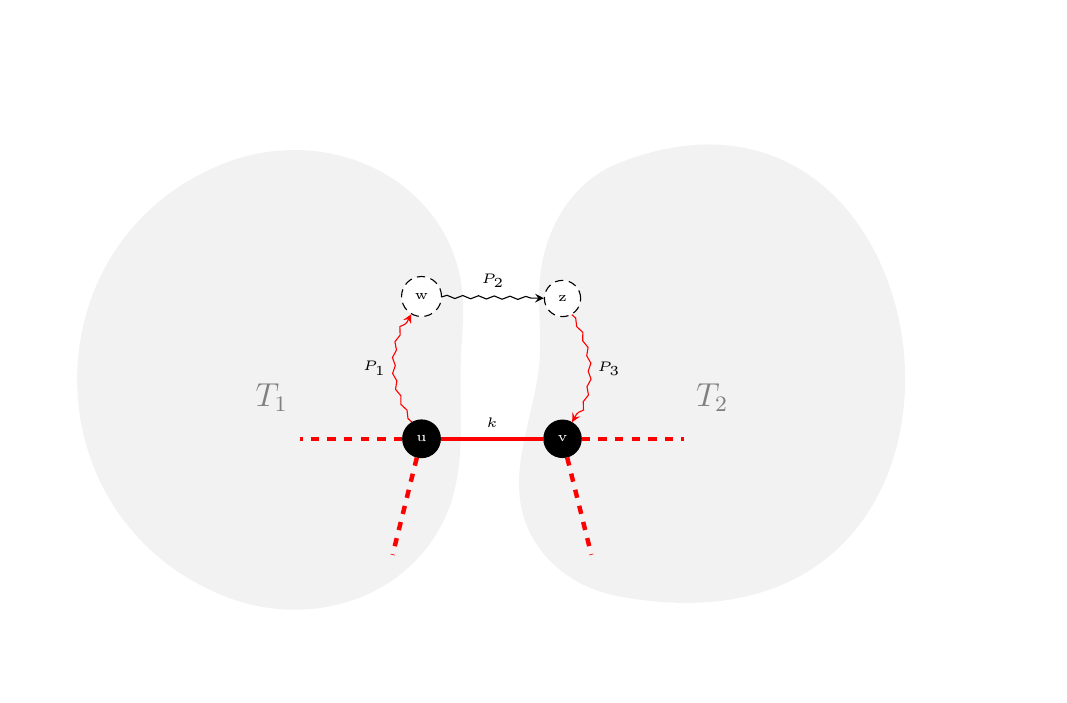
\begin{tikzpicture}[auto, node distance=1.3 cm]
      % Pre
      \begin{scope}[]
        \path[fill=black!5,use Hobby shortcut,closed=true]
        (-2.5, -2) .. (0.3,-1) .. (.5,1) .. (.5,2)  .. (-2.5,3.5);
        \path[fill=black!5,use Hobby shortcut,closed=true]
        (2.5, -2) .. (1.3,-1) .. (1.5,1) .. (1.5,2)  .. (2.5,3.5);

        \node[terminal] (u) at(0, 0) {u};
        \node[subgraph, above left= 0.05cm and 1.4cm of u] {$T_1$};
        \node[steiner, densely dashed] (w1) [above=of u] {w};
        
        \node[terminal] (v) [right= of u] {v};
        \node[subgraph,above right= 0.05 and 1.4cm  of v] {$T_2$};
        \node[steiner, densely dashed] (w2) [above=of v] {z};
        \node (sga) [left= of u] {};
        \node (sga2) [below left= 1.3 and 0.1 of u] {};

        \node (sgb) [right=  of v] {};
        \node (sgb2) [below right= 1.3 and 0.1 of v] {};

        
        
        %Edges
        \draw[selected] (u) edge node {$k$} (v);
        \draw[dashed, selected] (u) to (sga);
        \draw[dashed, selected] (u) to (sga2);

        \draw[dashed, selected] (v) to (sgb);
        \draw[dashed, selected] (v) to (sgb2);

        \draw (u) edge[snake it, red, bend left] node[text=black] {$P_1$} (w1);
        \draw (w1) edge[snake it] node {$P_2$} (w2);
        \draw (w2) edge[snake it, red, bend left] node[text=black] {$P_3$} (v);
      \end{scope}

      % \draw [->,decorate, thick,
      % decoration={snake,amplitude=.4mm,segment length=2mm,post length=1mm}]
      % (4,0) -- node [above=1mm,midway,text width=3cm, sloped, align=center] {}
      % (6,0);
      % Post      

  \end{tikzpicture}
  \caption{The optimal solution, $T = T_1 \cup T_2$ connected by $(u,v)$.
    Since $c(u,v) \geq B(u,v)^{-(u,v)}$,
  the simple path $P_2$ has cost no larger than $(u,v)$ and can replace it in $T$.}
  \label{fig:red:test:sd:thm}
\end{figure}

\subsubsection{Non-Terminals of Degree 3}
\label{sec:red:test:deg3}
Another bottleneck distance based test,
also proved valid for the PCSTP in \cite{uchoa2006reduction},
is the \textit{non-terminals of degree 3 test}.
\begin{theorem}[Non-Terminals of Degree 3 Test]\label{thm:ntd3}
  Let $u$ be a vertex with degree 3 in $G = (V, E, c, p)$,
  and let $v$, $w$, and $z$ be its adjacent
  vertices. If we have
  $$\min\left(B(v,w) + B(v,z), B(w,v) + B(w,z),  B(z, v)+ B(z, w)\right) \leq
  c_{uv} + c_{uw} + c_{uz}$$
  then there exists an optimal solution to $G$ where $u$ has degree of
  \textit{at most} 2, that is $|\delta(u)| \leq 2$. Thus $u$ and its three edges, can be replaced by
  the edges $\{(v, w), (w,z), (z,v)\}$ with costs
  $$c_{vw} = c_{vu} + c_{uw},\quad c_{wz} = c_{wu} + c_{uz},\quad c_{zv} = c_{zu} + c_{uv}\mathnormal{.}$$
\end{theorem}
\begin{proof}   
  W.l.o.g. consider the case where $B(v,w) + B(v,z) \leq c_{uv} + c_{uw} + c_{uz}$,
  and let $T$ be an optimal solution which contains $(u,v)$, $(u,w)$, and $(u,z)$.

  Let $P_1 = (v, ..., w)$ be the simple path with Steiner distance
  $$sd(P_1) = B(v,w)$$
  and similarly let $P_2 = (v, ..., z)$ be the simple path with Steiner distance
  $$sd(P_2) = B(v,z)\mathnormal{.}$$
  This gives us the situation in Figure (\ref{fig:red:test:ntd3:thm}). Note that $u$ may be a part of either paths.

  Let $T_v$, $T_w$, and $T_z$ be the subtrees of $T$ obtained by
  removing the edges adjacent to $u$ from $T$, and construct a new solution with
   total cost no-larger than $T$ as,
   $$T' = T_v \cup T_w \cup T_z \cup P_1 \cup P_2\mathnormal{.}$$
   We must have $|\delta_{T'}(u)| \leq 2$. If we had $|\delta_{T'}| = 3$ then
   we would have
   $$P_1 = \left[v, (v,u), u, (u,w), w \right]$$
   and
   $$P_2 = \left[v, (v,u), u, (u,z) z \right]$$
   giving us
   $$B(v,w) + B(v, z) = sd(P_1) + sd(P_2) = 2 c_{vu} + c_{uw} + c_{uz} > c_{vu} + c_{uw} + c_{uz}$$
   which is a contradiction to our original assumption that
   $$B(v,w) + B(v,z) \leq c_{uv} + c_{uw} + c_{uz}\mathnormal{.}$$
   Thus $T'$ is an optimal solution to $G$ with $|\delta_{T'}(u)| \leq 2$.
\end{proof}
\begin{figure}[h!]\centering
    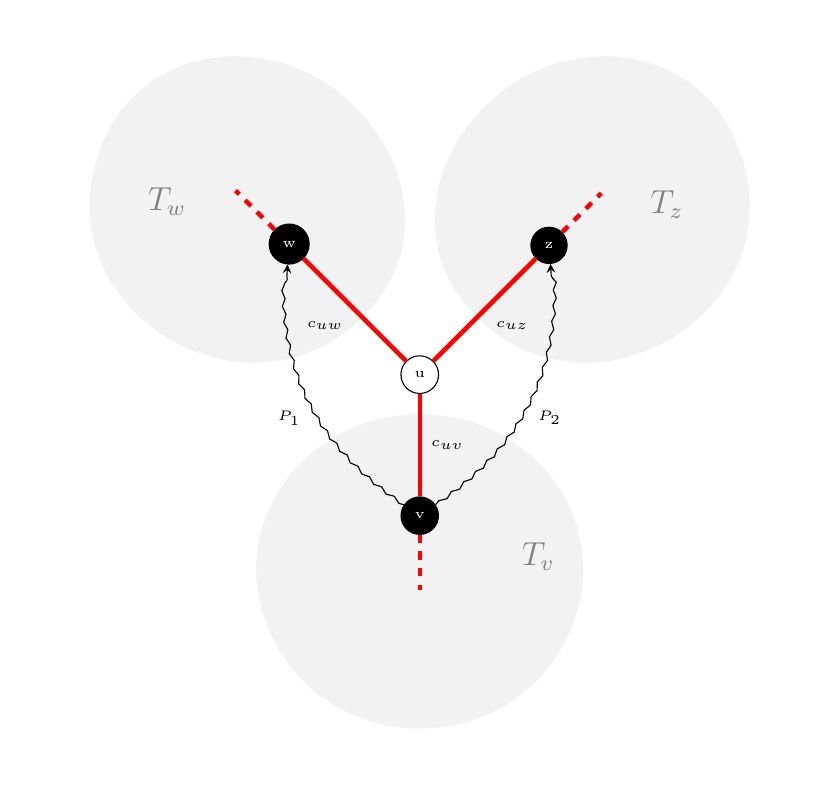
\begin{tikzpicture}[auto, node distance=1.3 cm]
      % Pre
      \begin{scope}[]
        \path[fill=black!5,use Hobby shortcut,closed=true]
        (-0.5, 1) .. (-4, 3) .. (-0.5,3);
        \path[fill=black!5,use Hobby shortcut,closed=true]
        (.5, 1) .. (4,3) .. (.5,3);
        \path[fill=black!5,use Hobby shortcut,closed=true]
        (0, -.5) .. (-2,-3) .. (2,-3);

        \node[steiner] (u) at(0, 0) {u};
        \node[terminal] (w) [above left=1.3 and 1.3 of u] {w};
        \node[terminal] (v) [below= of u] {v};
        \node[terminal] (z) [above right= 1.3 and 1.3 of u] {z};

        \node[subgraph, above left= 0.05cm and 1 cm of w] {$T_w$};
        \node[subgraph,above right= 0.05cm and 1 cm of z] {$T_z$};
        \node[subgraph, below right= 0.05cm and 1 cm of v] {$T_v$};
        
        \node (sgw) [above left= 0.7 of w] {};
        \node (sgv) [below= 0.7 of v] {};
        \node (sgz) [above right = 0.7 of z] {};
        
        %Edges
        \draw[selected] (u) edge node {$c_{uv}$} (v);
        \draw[selected] (u) edge node {$c_{uw}$} (w);
        \draw[selected] (u) edge node[swap] {$c_{uz}$} (z);
        \draw[dashed, selected] (v) to (sgv);
        \draw[dashed, selected] (w) to (sgw);
        \draw[dashed, selected] (z) to (sgz);

        \draw (v) edge[snake it, bend left] node[text=black] {$P_1$} (w);
        \draw (v) edge[snake it, bend right] node[swap,text=black] {$P_2$} (z);
      \end{scope}

      % \draw [->,decorate, thick,
      % decoration={snake,amplitude=.4mm,segment length=2mm,post length=1mm}]
      % (4,0) -- node [above=1mm,midway,text width=3cm, sloped, align=center] {}
      % (6,0);
      % Post      

  \end{tikzpicture}
  \caption{Non-Terminal of $|\delta(u)| = 3$ which connects the subtrees $T_v$, $T_w$, and $T_z$. The simple paths $P_1$ and $P_2$ provide an
     alternate way of reconnecting $T$ with at least as good cost.}
  \label{fig:red:test:ntd3:thm}
\end{figure}

\subsection{Summary of Usage}

\section{Primal Heuristics}

\section{Exact Algorithms}
%%% Local Variables:
%%% TeX-master: "report"
%%% reftex-default-bibliography: ("lit.bib")
%%% End:


\bibliographystyle{plainnat}
\bibliography{lit.bib}
\end{document}
